\subsection{Chap 1 } \label{chap1}

\begin{equation}
    \sigma = \frac{n e^2 \tau}{m^*}
\end{equation}


At it is a monovalent metal and the FCC-Unit cell contains 
4 atoms the concentration of the conduction electrons $N$ can be
calculated as:
$$N =\frac{4}{a^3} = $$

So for the collision time $\tau$ follows:

$$\tau = \frac{\sigma \cdot m^* \cdot a^3}{4e^2}$$

For a thin metal wire with a length of $10 \, cm$, a square cross section with 
a side of $0.1 \, mm$ and a potential difference along the wire of $0.2 \, V$

The electric field $E$ in the wire can be calculated as: 

$$E = \frac{U}{L} = 2 \frac{V}{m}$$

And for the drift velocitiy follows:

$$v_D =  -\frac{e \tau}{m^*} \cdot E$$

\subsubsection*{Fermi}

\begin{equation}
    f(E) = \frac{1}{e^{(E-E_F)/kT}+1}
\end{equation}

\begin{figure}[H]
    \centering
    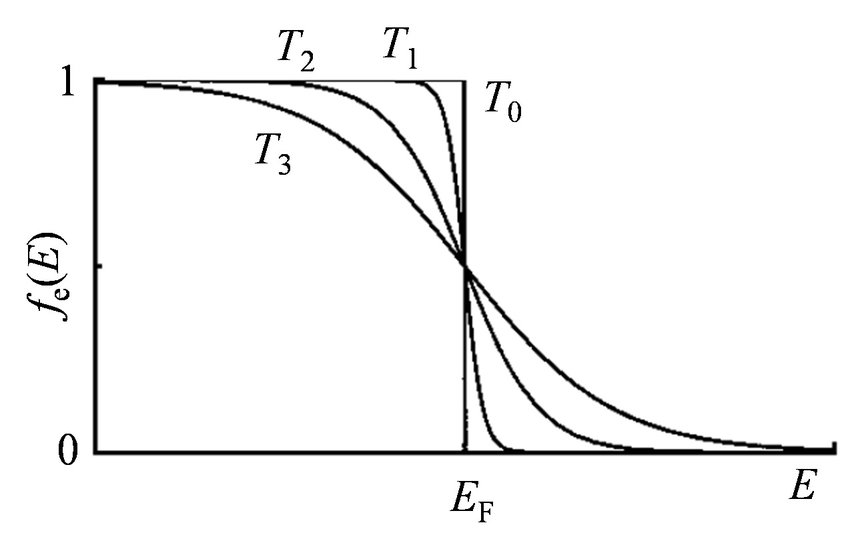
\includegraphics[width=0.5\linewidth]{Graphics/Chapter1/Fermi-Dirac-distribution.png}
    \caption{Fermi-Dirac distribution function at different temperatures: T3> T2>T1
     (and T0 = 0 K). At the absolute zero temperature (T0), the probability of an 
     electron to have an energy below the Fermi energy EF is equal to 1, while the 
     probability to have higher energy is zero.}
    \label{}
\end{figure}


\begin{figure}[H]
    \centering
    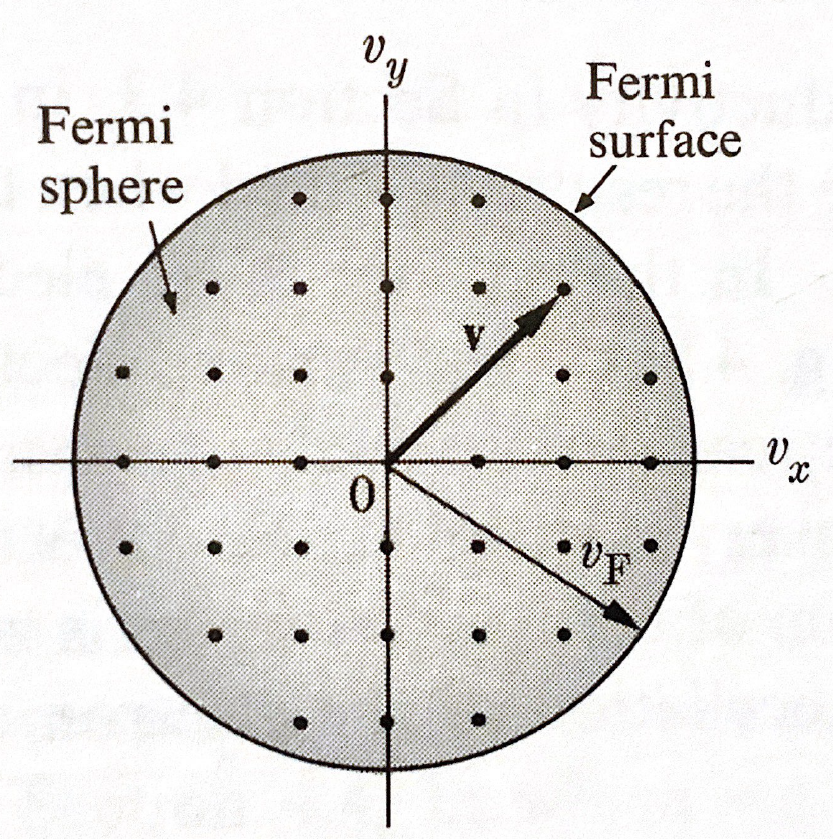
\includegraphics[width=0.4\linewidth]{Graphics/Chapter1/Fermi_Sphere.png}
    \caption{The Fermi surface and the Fermi sphere \cite[asdfadf]{elementary_SSP} }
    \label{}
\end{figure}

\subsubsection*{Cyclotron}
\begin{equation}
    -e (\vec{v} \times \vec{B}) =  m \frac{d\vec{v}}{dt}
\end{equation}

\subsubsection*{Plasma Frequency}

\begin{equation}
    w_P = \frac{Ne^2}{\epsilon_L m^*}
\end{equation}